%&pdflatex
\documentclass[11pt]{article}

\usepackage{geometry}                % See geometry.pdf to learn the layout options. There are lots.
\usepackage{listings}
\usepackage{graphicx}
\geometry{letterpaper}                   % ... or a4paper or a5paper or ...

\usepackage{hyperref}
\usepackage{bookmark}

\setlength{\parindent}{0pt}
\setlength{\parskip}{\baselineskip}%

\title{Programming Applications (PRA) \\ Minor Coursework Exercise 3 \\
``You'll Never Code Alone'' (2.5\%)}
%\author{Martin Chapman (martin.chapman@kcl.ac.uk)}
\date{}                                           % Activate to display a given date or no date

\begin{document}
\maketitle
%\section{}
%\subsection{}

%\vspace{-10mm}

\textbf{Please read the document marked `Q\&A Lab Projects and Pair Programming' carefully, before attempting any lab project. It contains important information on how to complete each minor piece of coursework, and is updated regularly. You will be asked to officially declare that you have read this document prior to submission. False declarations are taken seriously by both the department and by the college.}

\emph{This lab project counts for 2.5\% of your mark for the PRA minor coursework assessment, and is the third of four.}

\emph{The release weeks for this assignment start 20th February, at 23:55, and end 5th Match, at 23:55. All submissions must occur before the end of the second release week.}

\emph{If you have any questions about the structure of this assessment, please follow the `Additional Support' steps listed on KEATS.}

\textbf{You must select and work with a new partner for this piece of work}

The aims of the third lab project are as follows:

\begin{enumerate}
	
	\item To better understand, and critique, the model-view-controller (MVC) design pattern;
	
	\item To practice further with the use of widgets (components) and event handlers;
	
	\item To work with new components, and other aspects of Swing, such as the dropdown box and the File Chooser.

\end{enumerate}

In this specification, you will be guided towards a code structure that is consistent with (one flavour of) the model-view-controller (MVC) design pattern. This pattern, like all others, has benefits, but also drawbacks. As such, you may find yourself implementing things in a way that does not always feel natural. This is important, as it will allow you to fully comprehend the implications of using (this flavour of) the MVC pattern. Your TA will ask you about your experiences with MVC during your assessment.

An example of something that may not feel natural is the following. You will be asked to create (at least) the following classes: \texttt{Squad} and \texttt{Player} (part of the model) and \texttt{Fantasy} (part of the view). To ensure you stick closely to (this flavour of) the MVC design paradigm, there should be \textbf{no} references to the view (\texttt{Fantasy}) in the model (e.g. the \texttt{Squad} and \texttt{Player} classes) and vice-versa (no references to the model (e.g. the \texttt{Squad} and \texttt{Player} classes) in the view (\texttt{Fantasy})). In reality, when developing in accordance with the MVC paradigm, one might relax this constraint, but in this assignment we will not, in order to draw attention to the implications of the pattern. In addition, this separation will emphasise the difference between the model and the view and emphasise the role of the controller.

If you wish to deviate from the details of the specification given in the remainder of this document you may do so, as long as you still deliver the required functionality (in an equally efficient way), and retain the strict separation between the model and the view detailed in the previous paragraph.

\section{Domain Description}
\label{sec:domain}

\emph{Fantasy Football} (the sport that you play predominantly with your feet, not the sport that involves Beyonc{\'e} appearing at half time (not that there's anything wrong with Beyonc{\'e})) allows sports enthusiasts and nerds alike to choose a squad of 15 players, and field 11 of these players each week to play in a fictional team. Using a points system, the performance of the players in a fantasy manager's fictional team, in real life, then impacts the score of the manager, every week. In this project, we will \emph{not} focus on Fantasy Football scoring. 

The selection of a squad, and the selection of a team, is managed by a a graphical user interface. A fantasy manager can select two goalkeepers, five defensive players, five midfield players and three attacking players as part of their squad. The interface facilitates this selection, and then allows the manager to choose eleven of the fifteen players to `start' each week, with the remaining four players sitting on a fictional bench. Choosing which players start is done (in part) by selecting a team formation. An example of this is shown in Figure \ref{fig:real}, where the team formation chosen is `3-4-3' (3 defensive players, 4 midfield players and 3 attacking players) resulting in two defensive players and one midfield player sat on the bench, along with the second goalkeeper. Team formation does not directly affect the choice of goalkeeper, which we will assume, in this project, does not change (i.e. the same goalkeeper is always sat on the bench regardless of the formation).

\begin{figure}[htbp]
\begin{center}
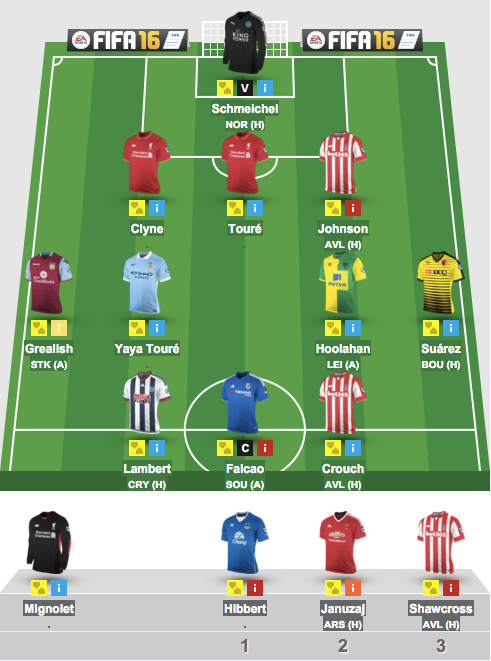
\includegraphics[width=230pt,height=300pt]{/Library/Server/Web/Data/Sites/webserver/PRA/distribute/CSnUsTh4/Assignment3Images/real.jpg}
\caption{An example Fantasy Football GUI, showing a team formation of `3-4-3' (we will not be aiming for a GUI of this complexity).}
\label{fig:real}
\end{center}
\end{figure}

In this project we will build a GUI to support squad selection and team formation, and do so adhering to (a specific flavour of) the MVC design pattern, which includes the model-view separation constraint given at the start of this document. 

\section{Setting up the packages}

Create a new \emph{project} in your chosen IDE. Inside this project, create a new \emph{package} named according to a concatenation of your first name, and the first name of your partner ($<$partnerApartnerB$>$). So, if Martin Chapman and Steffen Zschaler were embarking on this exercise, our project would contain a package called \emph{steffenmartin}. The order of names here is unimportant, but it is essential that you name your top-level package in this way, in order to identify your association with your partner to us.

Inside this package, create three \emph{subpackages} called \emph{model}, \emph{view} and \emph{controller}, respectively. After creating the \emph{model} subpackage (for example) its name, in most IDEs, should appear in the package or project view as $<$\emph{partnerApartnerB}$>$\emph{.model}, with $<$\emph{partnerApartnerB}$>$ naturally replaced with your first name, and that of your partner. If you locate the actual \emph{folder structure} created in your filesystem by your IDE for this project, you should now find a \emph{model} folder inside a $<$\emph{partnerApartnerB}$>$ folder. The same should be true after creating the other two subpackages.

\section{The Model}
\label{sec:model}

Place all the classes constructed in this section inside the \emph{model} subpackage.

Our model will hold data about a fantasy squad, in an appropriate structure, completely independently from the view. 

First, you will need to create a \texttt{Player}. A \texttt{Player} should have a \texttt{name}, although because this name may not be unique, players should also have an \texttt{ID}, which should be unique to each \texttt{Player} object. Next, a \texttt{Player} should be associated with an image \texttt{path}, that specifies a location on the hard drive of the computer where your Java application is running, where an image of that player exists. For example, if this field holds the value `schmeichel.jpg', this would imply that an image for this \texttt{Player} exists inside your project folder. The default value for the \texttt{path} attribute should be `None', or another recognisable value. Add getters and setters for these attributes as appropriate.

Finally, there should be a way of recording the role of a \texttt{Player} (goalkeeper, defender, midfielder or striker). A natural way to do this is to create four \emph{specialisations} of \texttt{Player}: \texttt{Goalkeeper}, \texttt{Defender}, \texttt{Midfielder} and  \texttt{Striker}, but there are other ways to record a player's role. However you choose to record the role of a \texttt{Player} ensure that the default value in the \texttt{name} attribute reflects the player's role. For example, if a \texttt{Player} is a goalkeeper, the initial value in the name attribute should be `Goalkeeper'.

For debugging purposes, it might be useful to ensure that when a \texttt{Player} object is printed, useful information about that player is shown on the terminal (such as their ID). 

Next, your model should hold information about a \texttt{Squad}. A \texttt{Squad} consists of a set of \texttt{goalkeepers}, \texttt{defenders}, \texttt{midfielders} and \texttt{strikers}. When a squad is \texttt{generated}, these sets should be filled with an appropriate number of \texttt{Player}s, as given in the Domain Description (Section \ref{sec:domain}). Initially, these \texttt{Player}s will simply be \emph{placeholders} (i.e. they will have no name (except the default name, discussed above) and no image path (again, except the default), as both these pieces of information are yet to be specified by the user). Add appropriate getters for these sets. Finally, a \texttt{Squad} should offer the ability to \texttt{search} for a player by \texttt{ID}.

\section{The View}

Place all classes constructed in this section inside the \emph{view} subpackage.

\subsection{Setting up the GUI}
\label{sec:setting}

Create a class for your view called \texttt{Fantasy}. The initial state of your view should look similar to the Frame mockup shown in Figure \ref{fig:view2}. In this view, we can see the visual representation of the player placeholders mentioned in Section \ref{sec:model}, with a text field that shows the default \texttt{name} value, and a button that prompts the user to add a picture of the player (because one does not yet exist), with a suitable symbol such as a `+'.  

\begin{figure}[htbp]
\begin{center}
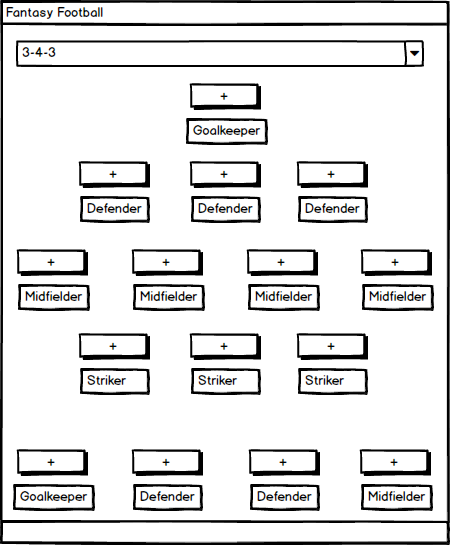
\includegraphics[width=240pt,height=300pt]{/Library/Server/Web/Data/Sites/webserver/PRA/distribute/CSnUsTh4/Assignment3Images/view2.png}
\caption{An overview of how your \texttt{Fantasy} frame should appear, after a team formation has been selected, and before any information is entered by the user. Players that are positioned without any information are known as placeholders.}
\label{fig:view2}
\end{center}
\end{figure}

When the program first runs, a new \texttt{Squad} should be \texttt{generate}d\footnote{We won't consider the notion of saving a team, in this project. Instead, each run of the program will constitute a fresh team generation.}. However, when the view (the \texttt{Fantasy} frame) is first loaded, we won't show any player placeholders for this squad. Instead, the only thing that should appear when the view is first loaded from Figure \ref{fig:view2} is the dropdown box, which should read `Select formation' (Figure \ref{fig:view1}). The team placeholders will then be shown once the first formation is selected. This dropdown box will be used to move the players in our view into different formations. The formations that your program should support, and thus which other entries the dropdown box should contain, is provided on KEATS. The part of the frame containing the team formation dropdown box I will refer to as the \emph{header}.

\begin{figure}[htbp]
\begin{center}
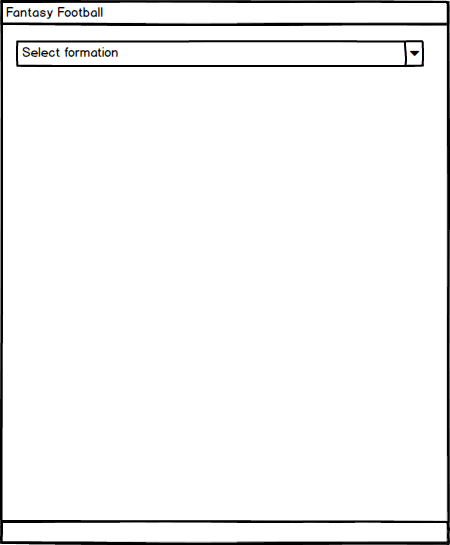
\includegraphics[width=240pt,height=300pt]{/Library/Server/Web/Data/Sites/webserver/PRA/distribute/CSnUsTh4/Assignment3Images/view1.png}
\caption{The first view that should be visible once your \texttt{Fantasy} frame is loaded.}
\label{fig:view1}
\end{center}
\end{figure}

Once the first team formation is selected, the centre of your frame (which I will refer to as the \emph{pitch}) should be filled with player placeholders (discussed shortly). To prepare for this, you should add four panels to the pitch, to hold the goalkeeper placeholder, the defender placeholders, the midfielder placeholders and the striker placeholders. These panels should be arranged so that the groups of players appear as shown in Figure \ref{fig:view2}, but of course before the first formation is selected, these panels will be empty. 

In a similar vein, the bottom of your frame should contain a single panel, which represents the \emph{bench}, and will contain players that do not feature on the pitch when a formation is selected. This is shown as the bottom row in Figure \ref{fig:view2}. Again, prior to selecting the first formation, this panel should be empty. 

As information is added about different players by the user, your view will evolve to look similar to what is shown in Figure \ref{fig:view3}. As you can see, several placeholders now contain information pertinent to each player, including their name and a picture. Therefore, over time, selecting a formation will not fill a panel with placeholders, but with actual player information. This is discussed further in Section \ref{sec:controller}.

\begin{figure}[htbp]
\begin{center}
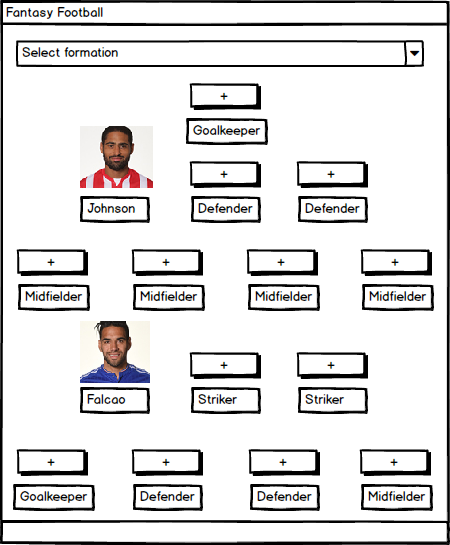
\includegraphics[width=240pt,height=300pt]{/Library/Server/Web/Data/Sites/webserver/PRA/distribute/CSnUsTh4/Assignment3Images/view3.png}
\caption{How your \texttt{Fantasy} frame should start to appear once a user starts adding information.}
\label{fig:view3}
\end{center}
\end{figure}

\subsection{Exposing functionality}
\label{sec:exposing}

Your view should expose the following functionality. Firstly, it should be possible to instruct the view to \texttt{add} a visual representation of each player (which may be a placeholder or actual player information) to each position on the pitch (\texttt{goal}, \texttt{defence}, \texttt{midfield} and \texttt{attack}), and to the \texttt{bench}. Each of these functions should accept a player ID, a player name and a player image path. While it might seem more natural to pass a complete \texttt{Player} object, remember we are purposefully not making any references to the model inside the view. 

Given a player ID, name and image path, a new panel should be added to the appropriate panel in either the pitch or the bench. I will refer to this new panel as a \emph{player panel}. To the bottom of this player panel, the player name should be added as a text field (I will refer to this as the \emph{player name}) so that it can be altered by the user. This text field will either contain the default value (e.g. Goalkeeper), as shown in Figure \ref{fig:view2}, or the name given to this player by the user (as shown for some players in Figure \ref{fig:view3}). To the centre of this player panel the image referenced by the image path (Figure \ref{fig:view3}) should be added. If the value in the image path is the default of  `None' (i.e. the player is still a placeholder), then rather than trying to show an image in the centre of the panel, a button should be shown that is designed to prompt the user to add a picture (as discussed in Section \ref{sec:setting}). I will refer to this button as the \emph{image prompt}. Importantly, you should attribute the player's ID to this player panel (perhaps by using the method \texttt{setName}) and to the player name and the image prompt, for future reference.

Next, it should be possible to instruct the view to \texttt{update} both the name and the image in an existing player panel, based upon a supplied player ID and either a new name or an object representing a path to a new image. When updating the image in a player panel, you should check whether an image prompt exists on that panel and if it does, it should be removed (i.e. it should only be possible to add an image to a player once).

Finally, it should be possible to instruct the view to remove all player panels from both the pitch and from the bench.

\textbf{Important:} You should read up on the respective roles of the \texttt{Component} commands \texttt{revalidate} and \texttt{repaint}, and see where they will be needed in your solution to show changes to the view. 

\section{The Controller}
\label{sec:controller}

Place all classes constructed in this section inside the \emph{controller} subpackage.

In this project, our controller will take the form of two different event handlers: one for responding to button press events and dropdown box selections, and one for responding to updates in a text field. Create a \texttt{Controller} that is able to respond to both of these types of event. To your view, add a reference to the \texttt{Controller}.

In PRA Lecture 4, we saw a flavour of the MVC design pattern in which the view was \emph{implicitly} updated by changes to the model using another design pattern, the Observer pattern. Here, we are going to explicitly use the controller to mediated the interactions between the model and the view. Both methods are reasonable ways to achieve an MVC design, as both achieve a separation between the model and the view. Therefore, if you wish to utilise the Observer pattern for this project, you may do so. For this specification however, to your controller, add a reference to both the view (\texttt{Fantasy}) and the model (\texttt{Squad}). 

Because the \texttt{Controller} is an event handler, it should be registered with the elements of the view that trigger pertinent events: the dropdown box for selecting formations in the header, the text field in each player panel and the image prompt in each player panel. The following sections describe the actions the \texttt{Controller} should take when it receives events from these three (sets of) components:

\subsection{New team formation selected in the dropdown box}

For simplicity, when a new team formation is selected, it is recommended that your controller instructs the view to clear all current player panels (using the method defined in Section \ref{sec:exposing}). Then, your program should determine how many players to add to each section of the pitch and the bench, based upon the selected formation. Players should only be added from the model (i.e. the \texttt{Controller} should never make any new \texttt{Player} objects, unless the \texttt{Controller} is in charge of generating the initial squad, in which case new \texttt{Player}s should only be made once), to ensure the persistency of information added during the running of the program.

A recommended procedure for updating the team formation in the view after the player panels have all been cleared is as follows:

\begin{enumerate}

	\item Add one goalkeeper to the goalkeeper panel (which goalkeeper is unimportant).
	
	\item Add another goalkeeper to the bench (which goalkeeper is unimportant).
	
	\item Examine each relevant part of the formation information (e.g. the relevant parts of `3-4-3' are `343').
	
	\item For each component of the formation, get the relevant players from the model, add the correct number of players from this set to the relevant panel in the view (using the predefined methods detailed in Section \ref{sec:exposing}), then add any remaining players from this set to the bench. For example, for the first `3' in `343', three defenders should be added to the defenders panel on the pitch in the view, and the remaining two defenders from the squad should be added to the bench. Which three defenders are on the pitch, and which two are on the bench, is unimportant.

\end{enumerate}

\subsection{Player name modified in the text field}
\label{sec:namemod}

When a player name is modified in the view, the controller should locate the relevant player in the model, and make a similar update. To determine the ID of the player whose name was modified, the controller should examine the source of the modification event, and extract the player ID from the text field, which should have been priorly set as that text field's name (see Section \ref{sec:exposing}).

\subsection{Player image prompt pressed}

When a player image prompt is pressed, the controller should trigger the display of a File Chooser. This will allow the user to locate a desired player image on their computer in a familiar manner. Conduct the appropriate research to learn how to display a File Chooser in Java. Several sample images are provided on KEATS for you to experiment with.

Once a path to the desired image is obtained, pass it to the priorly defined method for updating a player image in the view (Section \ref{sec:exposing}), along with the player ID (which should be obtained in a similar manner to how it was obtained in Section \ref{sec:namemod}). 

\textbf{Optional:} When loading an image for a player, the name of the image file is often also that player's name. Therefore, when an image is loaded, do not only update the image shown in the relevant player pane, but also update the player's name to be the same as the name of the image file. You will have to remove the extension (e.g. `.jpg') and you should ensure the first character of the name is an upper case letter for aesthetics.

\section{Putting everything together}

You should now create a \texttt{Main} class, and place it directly within your $<$\emph{partnerApartnerB}$>$ package (i.e. not within any of the subpackages). 

Main should then, roughly, do the following:

\begin{enumerate}

	\item Create the view (\texttt{Fantasy}).
	\item Create the model (\texttt{Squad}).
	\item Create the controller, passing an instance of the view and the model.
	\item \texttt{Generate} a set of player placeholders in the \texttt{Squad} (this may happen inside your \texttt{Controller}).
	\item Give the view a reference to \texttt{Controller}
	\item Show the \texttt{Fantasy} frame.

\end{enumerate}

Once the \texttt{Fantasy} frame is loaded, you should be able to select your first formation, presenting a set of 15 player placeholders. Any names or pictures added to replace (parts of) these placeholders should remain when switching between formations.

\subsection{Submitting your work}

\textbf{Ensure your code is correctly annotated with Javadoc comments}, in addition to standard comments. This is something we will be expecting to see from now on.

If, once finished, you wish to submit your work to us for preliminary feedback, you should do so by following the `Additional Support' steps from Step 3.2 onwards (i.e. direct contact), in order to avoid sharing your solution with your peers unnecessarily.

If you are happy with your solution, then you should both submit \emph{identical} copies of it to KEATS, adhering to all the submission rules given in the Q\&A document referenced at the beginning of this project brief. Nothing should differ between the submissions, especially the ordering of the names in the top-level package (i.e. $<$\emph{partnerApartnerB}$>$ should be the order adopted by \textbf{both} students).

The folder you compress for submission should be your top-level package, or the first folder inside your project source. For this assignment, the top-level folder is $<$\emph{partnerApartnerB}$>$. Compress this folder directly, so that the file you submit is of the form $<$\emph{partnerApartnerB}$>$.\\ $<$compression\_extension$>$ (e.g. steffenmartin.zip). Do not include anything else in your submission except folders pertaining to your packages, and your raw Java source files. Submissions with extraneous folders (e.g. `src' or `bin' folders from an IDE, folders pertaining to version control software etc.) will be penalised.

\end{document}
